\documentclass{beamer}

\setbeamertemplate{bibliography item}{[\theenumiv]}

\usetheme{Madrid}
%\usecolortheme{seahorse}
\usepackage[brazil]{babel}
\usepackage[utf8x]{inputenc} % acentos diretamente do teclado
\usepackage[T1]{fontenc}
\usepackage{graphicx}
\usepackage{xcolor}
\usepackage{tikz}
\usepackage{listings}
%\usepackage{courier}
\usepackage[scaled=0.8]{beramono}

%Box color
%\setbeamercolor{block title example}{fg=blue!50,bg=blue!10}
%\setbeamercolor{block body example}{fg=blue,bg=blue!5}
%\setbeamercolor{block title example}{fg=blue,bg=purple}
%\setbeamercolor{block body example}{fg=blue,bg=blue!5}

\title[Programação Paralela]{Intel Cilk Plus}
\subtitle{Programação Paralela}
\author[Alexandre \and Jeremias \and Matheus]{Alexandre Lucchesi%
    \and Jeremias Moreira%
    \and Matheus Braga}
\institute[UnB]{%
    Departamento de Ciência da Computação\\
    Universidade de Brasília, Brasília -- DF\\[1ex]
    \texttt{alexandrelucchesi@gmail.com}\\
    \texttt{jeremias@aluno.unb.br}\\
    \texttt{matheus.mtb7@gmail.com}\\
}
\date[Outubro, 2014]{10 de outubro de 2014}


\lstset{%
    language=C,
    basicstyle=\ttfamily,
    breaklines=true,
    morekeywords={cilk\_for, cilk\_spawn, cilk\_sync, cilk, grainsize}
}

\newcommand\tinyfootnote[1]{%
  \setbeamertemplate{footnote}{%
    \parindent 1em\noindent%
    \raggedright
    \hbox to 1.8em{\hfil\tiny\insertfootnotemark}\tiny\insertfootnotetext\par%
  }%
  \footnote{#1}%
  \setbeamertemplate{footnote}[default]
}

\begin{document}

\begin{frame}[plain]
    \titlepage%
\end{frame}

\begin{frame}[shrink]{Sumário}
    \tableofcontents
\end{frame}


%\section{Introdução}
%\subsection{O que é}
%\begin{frame}{Introdução}
%    \begin{itemize}
%        \item Cilk Plus é ``dahora''~\cite{jeffers:2013}.
%    \end{itemize}
%\end{frame}

\section{História}
\begin{frame}{História do Cilk}
\begin{itemize}
    \item O MIT desenvolveu o Cilk: uma tecnologia para programação
    \textit{multithread};
    \item O Cilk generaliza a semântica do C e introduz novas construções
    sintáticas para permitir a expressão de paralelismo;
    \item \textbf{O programador} deve se concentrar em estruturar seus programas
    de forma a explorar o \textbf{paralelismo} e a \textbf{localidade};
    \item \textbf{O Cilk} deve ser responsável pelo \textbf{escalonamento de
    tarefas} (em tempo de execução) maximizando o desempenho em
    \textbf{diferentes plataformas}.
\end{itemize}
\end{frame}

\begin{frame}{História do Cilk}
\begin{itemize}
    \item Cilk-1: suporte eficiente a \textbf{\textit{work-stealing}};
    \item Cilk-5: extensões simples para \textit{multithread} em ANSI C\@;
    \item Cilk++: versão comercial para C++ que introduziu reduções de
    hiperobjetos como técnica eficiente em aplicações cuja programação é
    irregular (ex: simulações \textit{N-body}, \textit{tree search}, etc);
    \item Cilk Plus: adicionou extensões para matrizes e foi incorporado ao
    compilador da Intel~\footnote{Pouco tempo após o lançamento do Cilk Plus, a
    Intel tornou pública as especificações da linguagem, permitindo sua
    incorporação em outros compiladores. Atualmente, além dos compiladores Intel,
    o Cilk Plus pode ser encontrado em versões do \texttt{gcc} e
    do \texttt{clang} (de forma limitada).}.
\end{itemize}
\end{frame}

\section{Funções Principais}
\subsection{Cilk Plus in a nutshell\ldots}
\begin{frame}{Cilk Plus \textit{in a nutshell}\ldots}
\begin{itemize}
    \item Elementos básicos:
    \begin{itemize}
        \item \texttt{cilk\_for};
        \item \texttt{cilk\_spawn};
        \item \texttt{cilk\_sync}.
    \end{itemize}
    \item Redução com hiperobjetos;
    \item Notação matricial.
\end{itemize}
\end{frame}
\subsubsection{cilk\_for}
\begin{frame}[fragile]{\texttt{cilk\_for}}
\begin{itemize}
    \item Permite que as iterações sejam executadas em paralelo.
\end{itemize}
\begin{block}{Exemplo}
\begin{lstlisting}
void saxpy(float a, float x[], float y[], size_t n) {
    cilk_for (size_t i = 0; i < n; i++)
        y[i] += a * x[i];
}
\end{lstlisting}
\end{block}
\end{frame}

\begin{frame}[fragile]{\texttt{cilk\_for}}
\begin{columns}[T]
\begin{column}{0.5\textwidth}
\begin{itemize}
    \item A sintaxe do \texttt{cilk\_for} tem algumas limitações, pois deve ser
    possível computar o espaço de iterações antes de executar o \textit{loop};
    \item O \texttt{corpo} deve ser paralelizável;
    \item O tipo de \texttt{idx} deve ser um inteiro ou \textit{iterator} de
    acesso randômico (ex: um ponteiro);
    \item Em \texttt{cond} podem ser utilizados somente: ${ !=, <, >, >=, <= }$;
\end{itemize}
\end{column}

\begin{column}{0.5\textwidth}
\begin{block}{}
\begin{lstlisting}
cilk_for(idx = expr; cond; incr)
    corpo;
\end{lstlisting}
\end{block}
\begin{itemize}
    \item \texttt{incr} é composto de um limite (\texttt{lim}) e um passo que
    devem ser avaliados apenas uma vez (imutáveis);
    \item O incremento (ou decremento) pode ser expressado com ${ +=, -=, ++,
    --}$.
\end{itemize}
\end{column}

\end{columns}
\end{frame}

\begin{frame}[fragile]{\texttt{cilk\_for}}
\begin{itemize}
    \item Como forma de evitar sincronizações execivas, e por padrão, o 
    \texttt{cilk\_for} divide (\textit{tiles}) o espaço de iterações, fazendo 
    com que cada \textit{thread} execute um \textit{tile}.
    \item Para casos onde é necessário maior controle da granularidade,
    pode-se o utilizar o \textbf{\texttt{pragma cilk grainsize}} para
    especificar o tamanho de um \textit{tile}:
\begin{lstlisting}
#pragma cilk grainsize = 1
cilk_for (int i = 0; i < n; i++)
    a[i] = f(b[i]);
\end{lstlisting}
\end{itemize}

\end{frame}
{
\usebackgroundtemplate{%
\tikz[overlay,remember picture] \node[opacity=0.025, at=(current page.center)] {
   
\includegraphics[height=\paperheight,width=\paperwidth]{img/spawn.jpg}};
}
\subsubsection{cilk\_spawn}
\begin{frame}[fragile]{\texttt{cilk\_spawn}}
\begin{itemize}
    \item O \texttt{cilk\_spawn} cria e executa uma nova \textit{thread}
    de \textbf{forma assíncrona};
    \item Possui mecanismos que possibilitam a recuperação do valor de retorno
    da chamada~\footnote{Os argumentos passados para a função são
    avaliados antes do \textit{fork} (\textit{strict evaluation}).}:
\begin{lstlisting}
x = cilk_spawn f(*p++);
\end{lstlisting}
    \item É possível criar chamadas assíncronas de um conjunto de instruções
    através de \textbf{expressões lambda}:
\begin{lstlisting}
cilk_spawn [&]{
    for (int i = 0; i < n; i++)
        a[i] = 0;
} ();
\end{lstlisting}
\end{itemize}
\end{frame}
}
\subsubsection{cilk\_sync}
\begin{frame}{\texttt{cilk\_sync}}
\begin{itemize}
    \item O \texttt{cilk\_sync} consiste em um mecanismo de sincronização que se
    assemelha a um \textit{join}.
    \item O escopo de uma chamada \texttt{cilk\_sync} é a função inteira na qual
    foi declarada e existe uma chamada \texttt{cilk\_sync} implícita no final de
    cada função.
    \item Isso implica que todo o paralelismo criado com o Cilk Plus em
    determinada função, termina antes que ela retorne.
\end{itemize}
\end{frame}

\begin{frame}[fragile]{\emph{Not only} uma questão de estilo\ldots}
\begin{columns}[c]

\begin{column}{0.3\textwidth}
\begin{block}{Código}
% Bad style...
\begin{lstlisting}
...
cilk_spawn f();
cilk_spawn g();
...
cilk_sync;
...
\end{lstlisting}
\end{block}
\end{column}

\pause

\begin{column}{0.6\textwidth}
\begin{figure}
    \centering
    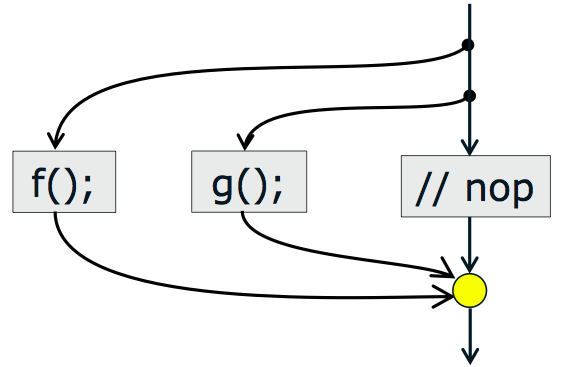
\includegraphics[width=\columnwidth]{./img/bad-style.png}
\end{figure}
\end{column}
\end{columns}
\end{frame}

\begin{frame}[fragile]{\emph{Not only} uma questão de estilo\ldots}
\begin{columns}[c]

\begin{column}{0.3\textwidth}
\begin{block}{Código}
% Good style...
\begin{lstlisting}
...
cilk_spawn f();
g();
...
cilk_sync;
...
\end{lstlisting}
\end{block}
\end{column}

\pause

\begin{column}{0.4\textwidth}
\begin{figure}
    \centering
    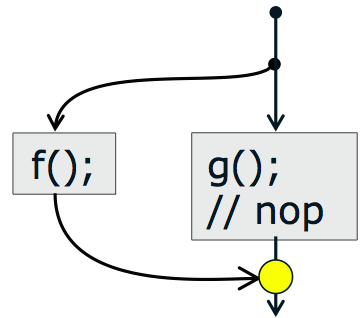
\includegraphics[width=\columnwidth]{./img/good-style.png}
\end{figure}
\end{column}
\end{columns}
\end{frame}

\subsection{Hiperobjetos}
\begin{frame}[fragile]{Hiperobjetos}
    Hiperojetos possibilitam acesso \textit{thread-safe} a objetos compartilhados, dando a cada \textit{thread} uma instância do objeto.
\begin{columns}[T]
\begin{column}{0.5\textwidth}
\begin{itemize}
    \item São em sua maioria redutores e fornecem uma operação que mecla dois \textit{views} para o redutor. 
\end{itemize}
\begin{footnotesize}
\begin{block}{}
\begin{lstlisting}
    cilk::reducer_opadd<float> sum = 0;
    ...
    cilk_for(size_t i = 1; i < n; i++){
// Atualiza a soma local.
        sum += f(i);
    }
// get_value() retorna a soma global.
    result = sum.get_value(); 
\end{lstlisting}
\end{block}
\end{footnotesize}

\end{column}

\begin{column}{0.4\textwidth}
\begin{footnotesize}
\begin{block}{Redutores}
Lists \\
\qquad list\_append \\
Listas \\
\qquad list\_append, list\_prepend \\
Mínimo e Máximo \\
\qquad max, max\_index, min, min\_index \\
Operadores Matemáticos \\
\qquad add, mul \\
Operadores bit-a-bit \\
\qquad and, or, xor \\
Concatenação de strings \\
\qquad string, wstring \\
Arquivos \\
\qquad ostream
\end{block}
\end{footnotesize}

\end{column}

\end{columns}
\end{frame}

\begin{frame}[fragile]{Hiperobjetos}
    Tais operações possibilitam a utilização de regiões compartilhadas sem o uso de \textit{locks}, com as seguintes características:
    \begin{itemize}
	    \item Funciona para qualquer operação de redução associativa.
	    \item As operações não precisam ser comutativas.
        \item O redutor não necessita ser uma variável local.
    \end{itemize}
\end{frame}

\begin{frame}[fragile]{Hiperobjetos}
    Hiperobjetos possuem diferentes sintaxes e comportamentos em C e C++.
\begin{columns}[T]
\begin{column}{0.4\textwidth}
\begin{tiny}
\begin{block}{C}
\begin{lstlisting}
CILK_C_REDUCER_OPADD(sum, int, 0);
CILK_C_REGISTER_REDUCER(sum);
cilk_for(int i = 0; i < 6021023; ++i) {
    REDUCER_VIEW(sum) += a[i];
}
CILK_C_UNREGISTER_REDUCER(sum);
printf("Soma: %d\n", REDUCER_VIEW(sum));
\end{lstlisting}
\end{block}
\end{tiny}
\end{column}

\begin{column}{0.4\textwidth}

\begin{tiny}
\begin{block}{C++}
\begin{lstlisting}
cilk::reducer_opadd<int> sum;
cilk_for (int i = 0; i < 6021023; i++) {
    sum += i;
}
printf("Soma: %d\n",sum.get_value());
\end{lstlisting}
\end{block}
\end{tiny}

\end{column}
\end{columns}
\end{frame}

\subsection{Notações Matriciais e Funções Elementares}

\begin{frame}{Notações Matriciais e Funções Elementares}
\begin{block}{}
\centering
    O Cilk Plus estende o C/C++ para utilizar Notações Matriciais e Funções 
    Elementares, o qual permite ao programador especificar seções de uma matriz 
    da qual será realizado o acesso. Tal notação auxilia o compilador na 
    realização de vetorização e autoparalelização.
\end{block}
\end{frame}

\subsubsection{Notações Matriciais}
\begin{frame}{Notações Matriciais}
\begin{block}{Expressões de Seção}
    Forma de selecionar múltiplos \textit{arrays} de elementos para operações de dados paralela.
\begin{block}{Sintaxe}
    [Início:tamanho:passo]
\end{block}
    A respectiva tripla representa uma sequência de valores subscritos a partir 
    do \textbf{início}, com $n$ elementos de \textbf{tamanho}, onde cada um 
    distancia-se pelo \textbf{passo}, utilizando a seguinte fórmula:
\begin{block}{}
    \centering
    \textit{inicio, inicio$+$passo, inicio$+$passo$*2$,$\ldots$, inicio$+$passo$*$(tamanho$-1$)}
\end{block}
\end{block}

\end{frame}

\begin{frame}{Notações Matriciais}
\begin{block}{Expressões de Seção}
    Expressões de Seção seguem as seguintes regras:
    \begin{itemize}
	    \item Se não há passo, o valor do mesmo é 1.
	    \item Se a tripla não contém expressões, o valor de início é $0$ e o 
	    valor de tamanho é o número de elementos contidos no \textit{array}.
	    \item Se o passo é negativo, o valor de início apontara para o índice mais alto.
	    \item Se o tamanho $\leq 0$, a sequência é vazia.
    \end{itemize}
\end{block}

\end{frame}

\begin{frame}[fragile]{Notações Matriciais}
\framesubtitle{Expressões de Seção}
    Cada Expressão de Seção possui um rank que ditam as regras de operações que
    podem ser realizadas com aquele \textit{array}.~\footnote{São diversas as
    regras a respeitos de Expressões de Seção e foge ao escopo do Seminário,
    que é uma apresentação superficial sobre a ferramenta, explorá-las}
\begin{small}
\begin{block}{Exemplos de Expressões de Seção}
    int *ponteiro; \\
    int Matriz[i][j]; \\ \pause
    ponteiro[:] = ...; // Não é uma operação válida por não haver tamanho declarado. \\ \pause
    matriz[:][:] = ...; // matriz bidimensional. \\ \pause
    ponteiro[1:5] = ...; // ponteiro[1],ponteiro[2], ... ponteiro[5]. \\ \pause
    matriz[0:5][0:7]; 	// Referem-se aos 35 elementos de uma matriz bidimensional. \\
\end{block}
\end{small}
\end{frame}
{
\renewcommand{\footnotesize}{\tiny} 

\begin{frame}[fragile]{Notações Matriciais}
\framesubtitle{Operações com Expressões de Seção}
    É uma operação paralela para modificar elementos da seção da matriz do lado
    esquerdo.\footnote{Se a operação do lado direito não se associa diretamente
    com os elementos do lado esquerdo, a substituição não é completa e o
    comportamento é indefinido}
\begin{scriptsize}
\begin{block}{Atribuição}
    a[0:10] = a[10:10];		// sem sobreposição; bem definida \\
    a[0:10:2] = a[1:10:2];	// sem sobreposição; bem definida \\
    a[0:10] = a[0:10] + 1;	// com sobreposição; bem definida\\
    a[0:10] = a[1:10]; 		// sobreposição imcompleta; comportamento indefinido \\
\end{block}
\pause
\begin{block}{Operações Aritméticas}
\begin{columns}
\begin{column}{0.17\textwidth}
\begin{tiny}
\begin{block}{}
    A[:] = 1.0;	\\
    A[0:3][0:3] = B[0]; \\
    C[:] = A[:] + B[:];	\\
\end{block}
\end{tiny}
\end{column}
\pause
\begin{column}{0.42\textwidth}
\begin{tiny}
\begin{block}{}
    C[20:10] = A[10:10] + B[0:10]; \\
    C[20:10][0] = A[10:10][2] + B[0:10][3];	\\
    C[0:9][0][0:9] = A[0][0:9][0:9] + B[0:9][0:9][4]; \\
\end{block}
\end{tiny}
\end{column}
\end{columns}
\pause
\begin{columns}
\begin{column}{0.75\textwidth}
\begin{tiny}
\begin{block}{}
    A[:] *= 2; \\ 
    A[:]++;	\\
    A[:] = B[:] == C[:]; \\
\pause
    A[0:2][0:2] = B[0:2]; // Erro! Problema quanto ao número de dimensões!\\
\end{block}
\end{tiny}
\end{column}
\end{columns}

\end{block}
\end{scriptsize}

\end{frame}
}
\begin{frame}[fragile]{Notações Matriciais}
\framesubtitle{Chamadas de função}
   A chamada de uma função utilizando uma expressão de seção mapeia chamadas com os elementos sucessivos da mesma.

\begin{block}{Função Escalar}
\begin{lstlisting}
void funcaoEscalarQualquer(int i) {
    printf ("%3d ", i);
}
\end{lstlisting}
\end{block}
\pause
\begin{scriptsize}
\begin{columns}
\begin{column}{0.4\textwidth}
\begin{block}{Versão escalar} 
\begin{lstlisting}
for(int i = 0; i < n; i++){
    funcaoEscalarQualquer(a[i]);
}
\end{lstlisting}
\end{block}
\pause
\end{column}
\begin{column}{0.55\textwidth}
\begin{block}{Versão escalar com notação matricial} 
\begin{lstlisting}
    funcaoEscalarQualquer(a[:]);
\end{lstlisting}
\end{block}
\end{column}

\end{columns}
\end{scriptsize}
\end{frame}

\begin{frame}[fragile]{Notações Matriciais}
\framesubtitle{Operações de Redução}
	Operações de redução em Notações Matriciais funcionam de forma similar
	aquelas existentes nas hiperoperações, sendo executadas para a seção
	estipulada do \textit{array}.

\begin{block}{Lista de Operações de Redução}
\begin{small}
\begin{small}
\begin{columns}
\begin{column}{0.45\textwidth}
\begin{itemize}
    \item \_\_sec\_reduce\_add
    \item \_\_sec\_reduce\_mul
    \item \_\_sec\_reduce\_max
    \item \_\_sec\_reduce\_min
    \item \_\_sec\_reduce\_max\_ind
\end{itemize}
\end{column}
\begin{column}{0.45\textwidth}
\begin{itemize}
    \item \_\_sec\_reduce\_min\_ind
    \item \_\_sec\_reduce\_all\_zero
    \item \_\_sec\_reduce\_all\_nonzero
    \item \_\_sec\_reduce\_any\_zero
    \item \_\_sec\_reduce\_any\_nonzero
\end{itemize}
\end{column}
\end{columns}
\end{small}
\end{small}
\end{block}
\end{frame}

%ESSE TÓPICO DEVERIA FICAR APÓS TODAS AS EXPLICAÇÕES E ANTES DOS EXEMPLOS - O QUE ACHAM???
\subsection{Serial Elision}
\begin{frame}[fragile]{\textit{Serial Elision}}
\begin{itemize}
    \item O Cilk Plus, de uma forma geral, é uma linguagem pouco intrusiva;
    \item Isso fica explícito quando se deseja, por exemplo, obter a versão
    serial (\textit{serial elision}) de um programa Cilk Plus: basta eliminar as
    palavras-chave \texttt{cilk\_spawn}, \texttt{cilk\_sync} e
    \texttt{cilk\_for};
    \item De forma trivial:
\begin{lstlisting}
#define cilk_spawn
#define cilk_sync
#define cilk_for for
\end{lstlisting}
    \item O resultado é um programa serial C/C++ válido.
\end{itemize}
\end{frame}

\subsection{Exemplos}
\begin{frame}{Exemplos}
\end{frame}

\begin{frame}{Análise Comparativa}
\section{Análise Comparativa}
\subsection{Gráfico de \protect\textit{Speedup}}
\end{frame}

\section{Aspectos da Ferramenta}
\subsection{Vantagens}
\begin{frame}{Vantagens}
\begin{itemize}
    \item Diretivas básicas bem definidas e de uso trivial;
    \item \textit{Syntactic sugar} para manipulação de \textit{arrays};
    \item Focada em otimizar resultados em processadores da
    Intel\textsuperscript{\textregistered};
    \item Implementa SIMD;
    \item Proporciona um meio onde o programador não precisa se preocupar com
    quase nada.
\end{itemize}
\end{frame}



\subsection{Desvantagens}
\begin{frame}{Desvantagens}
\begin{itemize}
    \item Dificuldade de se instalar;
% Esse ítem aqui acho que tá errado, já que ela usa Serial Elision e funciona de forma similar ao OPENMP
%    \item Muito invasiva, necessita de modificações no compilador e faz alterações na própria sintaxe.
    \item Manipulação de recursos (ex.: \textit{workers}) não é nativa da
    ferramenta.
% COMENTAR, MAS NÃO ESCREVER ISSO EXPLICITAMENTE - São necessárias verdadeiras gambiarras para modificar, por exemplo, o número de threads.
    \item Complicado de se otimizar.
\end{itemize}

\end{frame}


\section{Conclusão}
\begin{frame}%[allowframebreaks]
    \frametitle{Referências Bibliográficas}
    \tiny{\bibliographystyle{abbrv}}
    \bibliography{refs}
\end{frame}

\end{document}

